\documentclass[aspectratio=169,xcolor=dvipsnames,t]{beamer}
\usepackage[utf8]{inputenc}

\usepackage{amssymb}
\usepackage{amsmath}
\usepackage{rotating}
\usepackage{graphicx}
\usepackage[mathscr]{euscript}
\usepackage[dvipsnames,svgnames,table]{xcolor}
\usepackage{multicol}
\usepackage{multirow}
\usepackage{physics}
\usepackage[version=4]{mhchem}
\usepackage[spanish,es-nodecimaldot,es-tabla]{babel}
\usepackage{parskip}
\usepackage{hyperref}
\usepackage{csquotes}
\usepackage{wrapfig}
\usepackage{ragged2e}
\justifying

\usepackage{bookmark}

\usepackage{etoolbox}
\usepackage{textcase}
\makeatletter
\patchcmd{\beamer@Section}{\Section}{\Section{\MakeTextUppercase}{}{}}{}{}
\patchcmd{\beamer@Subsection}{\Subsection}{\Subsection{\MakeTextUppercase}{}{}}{}{}
\makeatother

\usepackage[backend=biber,citestyle=numeric-comp,bibstyle=apa,sorting=none]{biblatex}
\bibliography{ref}
\makeatletter
\RequireBibliographyStyle{numeric}
\makeatother

\newcommand{\be}{\begin{equation*}}
\newcommand{\ee}{\end{equation*}}
\newcommand{\ble}[1]{\begin{equation} \label{#1}}
\newcommand{\bae}{\begin{eqnarray}}
\newcommand{\eae}{\end{eqnarray}}
\newcommand{\pl}{\left(}
\newcommand{\pr}{\right)}
\newcommand{\kl}{\left[}
\newcommand{\kr}{\right]}

\setbeamertemplate{footline}[frame number]

\usetheme{Arguelles}

%%%%%%%%%%%%%%%%%%%% Opciones título %%%%%%%%%%%%%%%

\title{Comparación del Output Factor del VB respecto al TB}
%\subtitle{INCan}

\date{\today}
\author{Christopher López Ruiz}
\institute{INCan}

%%%%%%%%%%%%%%%%%%%%%%%%%%%%%%%%%%%%%%%%%%%%%%%%%%%%%%%%%%%%%%%%%%%

\begin{document}

\frame[plain,bg=fondo.jpg]{\titlepage}

\Section{Output Factor}

\begin{frame}
    \frametitle{Output Factor}

    \begin{itemize}
          \item  $D_{w}$ es la base de la experiencia y los ensayos clínicos actuales.
          \item La calibración se hace con referencia al agua.
    \end{itemize}

\end{frame}

\Section{15X}

\begin{frame}[standout]
      \centering\LARGE
      \textbf{\itshape\scshape Energía = 15X}
\end{frame}

\begin{frame}

      \vspace{1cm}

      \begin{figure}
            \centering
            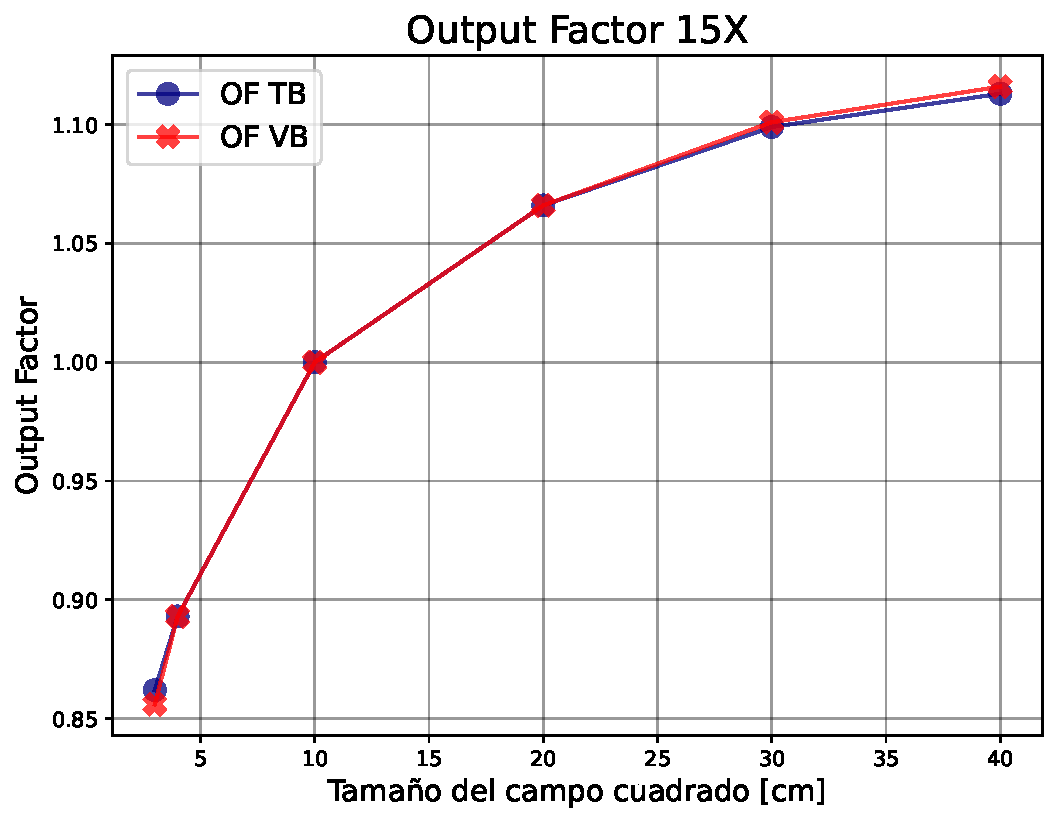
\includegraphics[width=1\textwidth]{15X_s.pdf}
      \end{figure}

\end{frame}

\Section{6X FFF}

\begin{frame}[standout]
      \centering\LARGE
      \textbf{\itshape\scshape Energía = 6X FFF} 
\end{frame}

\Section{Extras}

\begin{frame}[standout]
      \centering\LARGE
      \textbf{\itshape\scshape Extras}
\end{frame}

\End
\begin{frame}[standout,bg=white.png]
      \centering
\end{frame}

\end{document}